\documentclass[11pt]{article} % article, report, or book

\usepackage[margin=1.0in]{geometry}
%\usepackage[parfill]{parskip}    		% Activate to begin paragraphs with an empty line rather than an indent
\usepackage{graphicx}				% Use pdf, png, jpg, or eps§ with pdflatex; use eps in DVI mode
\graphicspath{{../figures/}}
\usepackage{amsmath}
\usepackage{color}
\usepackage[utf8]{inputenc} % allows for é
\usepackage{float} % allows for [H]

%=======================================================================================================
\title{\color{red}{We need a title, boi}}
\author{Luke Bury \& Don Kuettel}
%=======================================================================================================
\begin{document}
\maketitle
%=======================================================================================================
\section*{Introduction}
In 1885, a competition was held by Acta Mathematica in which participants were challenged to solve one of four outstanding math problems of time. Henri Poincaré, a prominent mathematician of the time, entered the contest and ultimately won. However, his submission contained a critical mistake that led to the discovery of homoclinic orbits and forever changed the future of dynamical mathematics. In the following report, this history and controversy of Poincaré's mistake are discussed, the mathematics that led to the discovery of homoclinic orbits are analyzed, and from this theory, real homoclinic orbits are found, simulated, and presented. 

\section*{The Competition}
As documented by Andersson and Barrow-Green \cite{Andersson1994,BarrowGreen1994}, in 1885, Acta Mathematica announced a mathematics competition to the world. This competition, sponsored by King Oscar II of Sweden, encouraged interested parties to make an attempt at solving one of four selected problems. Henri Poincaré, a prominant mathematician of the time (who was largely favored to win the competition) attempted the first problem, which essentially asked for a solution to the troubling $n$-body problem. However, Poincaré instead decided to attempt a subset of the $n$-body problem known as the three-body problem, since it was the first order of the problem remaining unsolved. To further simplify his initial effort, Poincaré restricted the three-body system in a manner known today as the Circular Restricted Three-Body Problem (CR3BP), which will be discussed further in the next section.

Poincaré's submission to the competition consisted of the culmination of several strands of his work from the previous decade, which included geometrical and analytical theory, integral invariants, and periodic solutions to dynamical systems. Poincaré applied these theories in an attempt to rigorously prove stability and find periodic solutions for the CR3BP. The competition judges immediately recognized the importance of Poincaré's submission and unanimoulsy crowned him the victor. However, around the time that his work was first being printed, a discussion with Lars Edvard Phragmén led to the discovery of an error within Poincaré's submission that held significant ramifications. The error was rooted in Poincaré's failing ``to take proper account of the exact geometric nature of a particular curve'' \cite{BarrowGreen1997}. In Theorem III of the paper's first, and flawed, edition, Poincaré claimed that a particular invariant curve was closed (Figure \ref{fig:curveIntersection1}(a,b)). He failed to consider that the curve could be self-intersecting (Figure \ref{fig:curveIntersection1}(c)). After realizing his mistake, Poincaré reworked his derivations to discover that the asymptotic surfaces are not closed, but instead, they intersect along infinitely many asymptotic trajectories. Ironically, this mistake cemented Poincaré's place among legendary mathematicians for his resulting discovery of \textit{doubly asymptotic}, or \textit{homoclinic}, points/orbits in the CR3PB and dynamical systems in general.  

\begin{figure}[H]
\centering
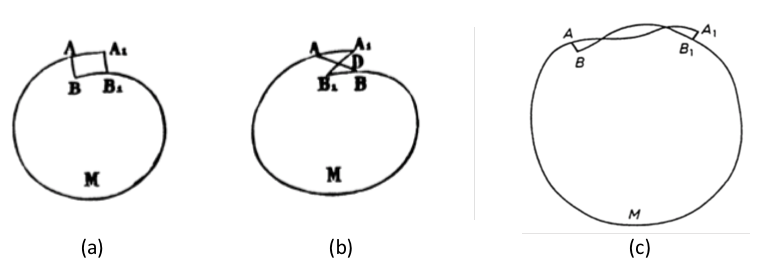
\includegraphics[width=5in]{curveIntersection1.png}\nonumber
\caption{(a) Diagrams of incorrectly closed invariant curves from the first edition of Poincaré's memoir. (b)Invariant curve with self intersection from Poincaré's corrected work \cite{BarrowGreen1997}}
\label{fig:curveIntersection1}
\end{figure}

\color{red}\textbf{MATH}\color{black}
%-----------------------------------------------------------------------------------------
%-----------------------------------------------------------------------------------------

\section*{Circular Restricted Three Body Problem and Applications}
\begin{itemize}
	\item \color{red}Description of CR3BP
	\item Application to find POs... manifolds... homoclinic orbits
	\item \color{black}
\end{itemize}

%-----------------------------------------------------------------------------------------
%-----------------------------------------------------------------------------------------
\section*{\color{red}{Periodic/Homoclinic Orbits}}
\begin{itemize}
	\item \color{red}Eq points and stability
	\item zero velocity curves
	\item POs and algorithm to find them
	\item manifolds and the algorithms
	\item PO stability ... eigenvalues of monodromy matrix; Poincare sections and their intersections ... homoclinic orbits
	\item Plotting and discussion of homoclinic orbits (piecewise)
	\item \color{black}
\end{itemize}

%-----------------------------------------------------------------------------------------
%-----------------------------------------------------------------------------------------
\section*{Conclusion}
\begin{itemize}
	\item \color{red}{Homoclinic orbits are cool/interesting, but for spacecraft applications they aren't very useful; Heteroclinic orbits are useful fa show}\color{black}
\end{itemize}

%=======================================================================================================
\newpage
\bibliographystyle{plain}
\bibliography{../bibliography/appm5460.bib}

\end{document}  